% !TEX root=/home/tavant/these/manuscript/src/manuscript.tex

\section{Impact of the radial boundary conditions on the oscillation}
  \label{subsec-BC}

  In \Cref{sec-DR-BC}, we discussed the choice of the radial wavenumber of the instability observed.
  Changing the radial electric boundary condition could affect the instability.
  Therefore, we discuss in this section  the impacts of the dielectric electrostatic boundary condition on the oscillation.
  We have seen in \Cref{sec-diel_layer} that the dielectric boundary did not affect the simulation results macroscopic.
  \Cref{fig-closswallosci} shows the radial evolution in the first few cells of the amplitude of the oscillation of the azimuthal electric field on the left, and the ion density on the right, with grounded (metallic) wall and dielectric wall.
  
  \begin{figure}[!hbt]
    \centering
    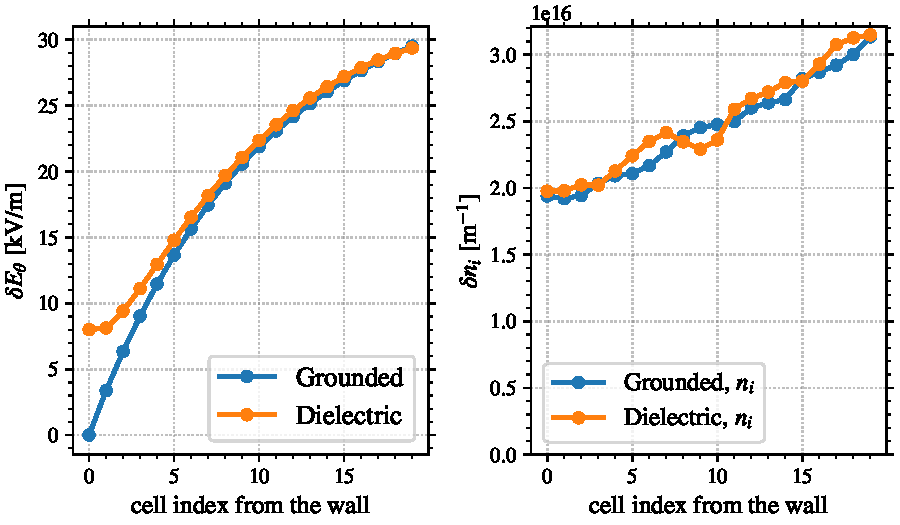
\includegraphics[width=\textwidth]{Ex_closewall.pdf}
    \caption{Radial evolution in the first cells of the amplitude of the oscillation of (left) the azimuthal electric field and (right) the ion density, with grounded (metallic) wall and dielectric wall.}
    \label{fig-closswallosci}
  \end{figure}
  
  We can see in \cref{fig-closswallosci} that the boundary condition does not affects the ion oscillations.
  This is consistent with the observation in \cref{subsec-kr} that the ion fluctuation was not affected by the wall.
  On the other hand, the azimuthal electric field has to go to zero when the wall is grounded.
  In contrast, using the dielectric boundary condition, the azimuthal electric field at the wall limit can be more than zero.
  Indeed, as seen in \cref{fig-indiel}, the amplitude of the azimuthal electric field decreases toward zero inside of the dielectric layer.
  
  Nevertheless, the difference in $E_{\theta}$ between the two boundary conditions quickly disappears inside the plasma domain.
  Indeed, after a dozen cells, corresponding to a few Debye lengths, the amplitudes of $\delta E_{\theta}$ are equal for both cases.
  Hence, the electrostatic boundary condition induces only minor differences in the instability and therefore the plasma discharge.
  
  